%versi 2 (8-10-2016)
\chapter{Landasan Teori}
\label{chap:teori}

\section{Big Data}
\label{sec:big data}

{\it Big data} adalah istilah yang menggambarkan kumpulan data dalam jumlah yang sangat besar, baik data yang terstruktur maupun data yang tidak terstruktur. Kumpulan data tersebut menyimpan informasi yang bisa dianalisis dan diproses untuk memberikan wawasan kepada organisasi atau perusahaan. Data-data tersebut berasal dari satu atau lebih sumber  dengan kecepatan yang tinggi dan format yang berbeda-beda. Karena ukuran dan keberagaman data, {\it big data} menjadi sulit untuk ditangani atau diproses jika hanya menggunakan manajemen basis data atau aplikasi pemrosesan data traditional~\cite{ishwarappa:01:bgintro}.\\


\begin{figure}[H]
    \centering  
    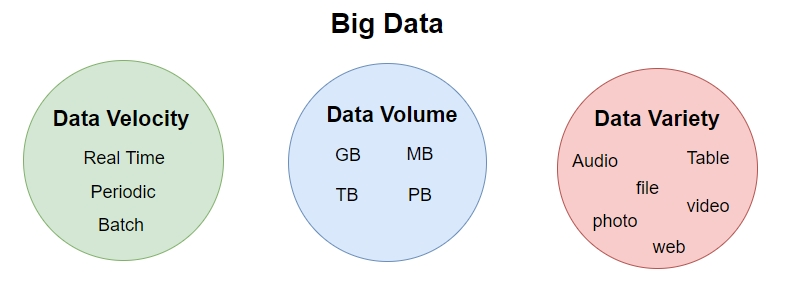
\includegraphics[scale=0.4]{bigdata}  
    \caption[Gambar {\it big data volume, velocity, variety} ]{Gambar {\it big data volume, velocity, variety}} 
    \label{fig:bigdata} 
\end{figure}

Berdasakan gambar diatas (Gambar ~\ref{fig:bigdata}), \textit{big data} memiliki lima karakteristik di antaranya ~\cite{ishwarappa:01:bgintro}:

\begin{enumerate}

\item {\it Volume}: {\it big data} memiliki jumlah data yang sangat besar sehingga dalam proses pengolahan data dibutuhkan suatu penyimpanan yang besar dan dibutuhkan analisis yang lebih spesifik.

\item {\it Velocity}: {\it big data} memiliki aliran data yang sangat cepat. Data baru dihasilkan dengan kecepatan yang tinggi dari satu atau lebih sumber. 

\item {\it Variety}: {\it big data} memiliki bentuk format data yang beragam baik terstruktur ataupun tidak terstruktur dan bergantung pada banyaknya sumber data. Data dapat berupa gambar, video dan tipe data lainya.

\item {\it Veracity}: {\it big data} mungkin mengandung data yang tidak akurat atau rusak. Kualitas  data dalam {\it big data} bisa berbeda-beda tergantung pada sumber. Analisis {\it big data} akan sangat dipengaruhi dengan keakuratan data.

\item {\it Value}: {\it big data} harus memiliki value. Tidak ada gunanya bila kita memiliki akses terhadap {\it big data}, tetapi data-data tersebut tidak memiliki nilai apapun. Data yang tidak memiliki nilai adalah data yang tidak berguna dan memakan biaya untuk disimpan.

\end{enumerate}

{\it Big data} sangat bermanfaat ketika diterapkan di berbagai macam bidang seperti bisnis, kesehatan, pemerintahan, pertanian dan lainya. Ketika organisasi mampu menggabungkan jumlah data besar yang dimilikinya dengan analisis bertenaga tinggi, organisasi dapat menyelesaikan tantangan dan masalah yang berhubungan dengan bisnis seperti:

\begin{enumerate}

\item Menentukan akar penyebab kegagalan untuk setiap masalah bisnis.

\item Menghasilkan informasi mengenai titik penting penjualan berdasarkan kebiasaan pelanggan dalam membeli.

\item Menghitung kembali seluruh risiko yang ada dalam waktu yang singkat.

\item Mendeteksi perilaku penipuan yang dapat mempengaruhi organisasi.

\end{enumerate}

\section{Algoritma Hierarchical Clustering}

\textit{Hierarchical Clustering Algorithm} (HCA) adalah metode analisis kelompok yang berusaha untuk membangun sebuah hirarki dengan mengelompokan data. Dengan mengelompokan data-data tersebut, data pada kelompok yang sama memiliki kemiripan yang tinggi dan data pada kelompok yang berbeda memiliki kemiripan yang rendah~\cite{veronica:02:bdhca}. Dalam reduksi data, \textit{cluster} yang merepresentasikan data-data pada \textit{cluster} tersebut akan diggunakan untuk mengganti data-data mentah~\cite{veronica:02:bdhca}. Seberapa efektif cara ini tergantung dengan sifat data yang ditangani. Data-data yang bisa dikelompokan kedalam \textit{cluster} yang berbeda akan sangat cocok dengan cara ini~\cite{veronica:02:bdhca}. Pada dasarnya HCA dibagi menjadi dua jenis yaitu \textit{agglomerative} (\textit{bottom-up}) dan \textit{devisive} (\textit{top-down})~\cite{veronica:02:bdhca}. Pendekatan \textit{agglomerative} berusaha membentuk sebuah hierarki dengan megabungkan \textit{cluster}. Setiap \textit{objek} akan dimasukan kepada \textit{cluster} tersendiri. Sebaliknya, pendekatan \textit{devisive} akan berusaha memecah \textit{cluster} untuk membentuk sebuah hierarki. Setiap objek berada pada satu cluster pada awalnya dan akan dipecah kepada cluster yang berbeda.\\

\begin{figure}[H]
    \centering  
    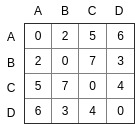
\includegraphics[scale=1]{matrix1}  
    \caption[Gambar matriks jarak]{Gambar matriks jarak} 
    \label{fig:matrix1} 
\end{figure}

\begin{figure}[H]
    \centering  
    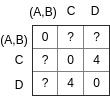
\includegraphics[scale=1]{matrix2}  
    \caption[Gambar matriks jarak]{Gambar matriks jarak} 
    \label{fig:matrix2} 
\end{figure}

Pada \textit{Agglomerative Hierarchical Clustering}, awalnya setiap objek akan dimasukkan kepada \textit{cluster} tersendiri. Matriks jarak digunakan untuk merepresentasikan jarak antara \textit{cluster}. Kemudian, dua buah \textit{cluster} yang memiliki similaritas tertinggi akan digabungkan menjadi satu \textit{cluster}. Similaritas antara cluster dapat dihitung dengan tiga metode yaitu \textit{single linkage}, \textit{complete linkage}, dan \textit{centroid linkage}~\cite{anil:03:afcd}. Pada Gambar ~\ref{fig:matrix1}, \textit{cluster} A dan  \textit{cluster} B akan digabung menjadi satu karena jarak antara keduanya adalah terkecil dibanding dengan yang lainnya. Gambar ~\ref{fig:matrix2} adalah hasil dari penggabungan \textit{cluster} A dan \textit{cluster} B dan matriks jarak harus dihitung kembali untuk mencari jarak baru antara \textit{cluster} baru dengan \textit{cluster} lainya. Penggabungan \textit{cluster} akan diulangi sampai tersisa satu \textit{cluster}. \textit{Agglomerative Hierarchical Clustering} akan hanya membutuhkan maksimal $n$ iterasi. Hasil dari penggabungan \textit{cluster} adalah sebuah hierarki. \textit{Dendrogram} sangat umum digunakan untuk menggambarkan proses \textit{Agglomerative Hierarchical Clustering}. Contoh \textit{dendrogram} dapat dilihat pada Gambar ~\ref{fig:dendo}.\\


\begin{figure}[H]
    \centering  
    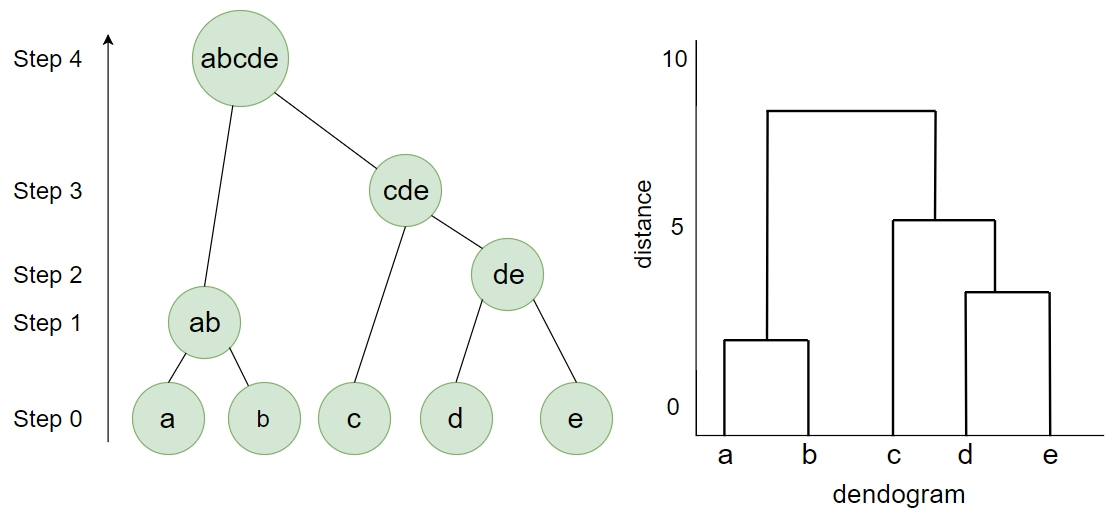
\includegraphics[scale=0.45]{dendo}  
    \caption[Gambar {\it dendrogram} ]{Gambar {\it dendrogram}} 
    \label{fig:dendo} 
\end{figure}


Berikut adalah penjelasan mengenai metode \textit{single linkage}, \textit{complete linkage}, dan \textit{centroid linkage}:

\begin{itemize}

\item \textit{Single linkage}: metode ini mencari jarak minimum dari perbandingan setiap anggota antara dua buah \textit{cluster}. Bila ada dua buah \textit{cluster} A dan B, maka setiap anggota pada \textit{cluster} A akan dihitung jaraknya kepada setiap anggota pada \textit{cluster} B. Kemudian jarak minimum antara anggota akan diambil sebagai hasilnya. Untuk menghitung jarak antara anggota dapat digunakan \textit{euclidean distance}, \textit{manhattan distance}, atau ruang metrik lainya. Ruang metrik yang digunakan disesuaikan dengan kebutuhan dan atribut dari data. Contoh \textit{single linkage} dapat dilihat pada Gambar ~\ref{fig:single}.

\begin{figure}[H]
    \centering  
    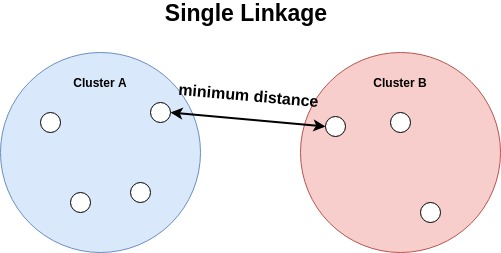
\includegraphics[scale=0.45]{single}  
    \caption[Gambar {\it single linkage} ]{Gambar {\it single linkage}} 
    \label{fig:single} 
\end{figure}

Berikut adalah rumus untuk \textit{single linkage}:

$$
min\{ d(a,b): a \in A, b \in B\}, 
$$
dengan $a$ dan $b$ merupakan anggota dari \textit{cluster} $A$ dan $B$.\\

\item \textit{Complete linkage}: metode ini adalah kebalikan dari metode \textit{single linkage}. Bila ada dua buah \textit{cluster} A dan B, maka setiap anggota pada \textit{cluster} A akan dihitung jaraknya kepada setiap anggota pada \textit{cluster} B. Kemudian jarak maksimum antara anggota akan diambil sebagai hasilnya. Contoh  \textit{complete linkage} dapat dilihat pada Gambar ~\ref{fig:complete}.

\begin{figure}[H]
    \centering  
    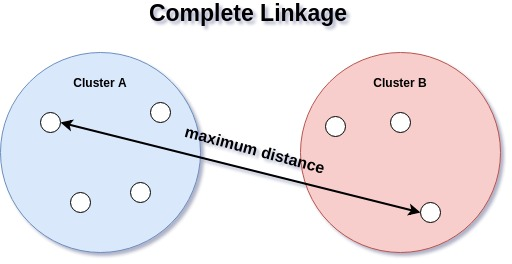
\includegraphics[scale=0.45]{complete}  
    \caption[Gambar {\it single linkage} ]{Gambar {\it single linkage}} 
    \label{fig:complete} 
\end{figure}

Berikut adalah rumus untuk \textit{single linkage}:

$$
max\{ d(a,b): a \in A, b \in B\}, 
$$
dengan $a$ dan $b$ merupakan anggota dari \textit{cluster} $A$ dan $B$.\\


\item \textit{Centroid linkage}: metode ini menghitung jarak antara \textit{centroid} dari dua buah \textit{cluster}.  \textit{Centroid} sebuah cluster didapatkan dengan menghitung rata-rata dari setiap atribute dari anggota pada \textit{cluster}. Contoh  \textit{centroid linkage} dapat dilihat pada Gambar ~\ref{fig:centroid}. 

\begin{figure}[H]
    \centering  
    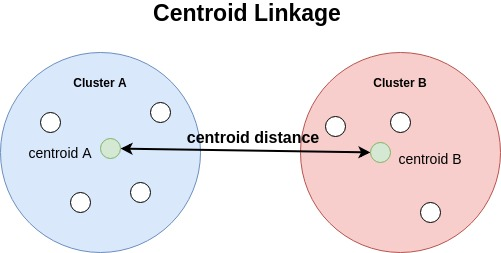
\includegraphics[scale=0.5]{centroid}  
    \caption[Gambar {\it centroid linkage} ]{Gambar {\it centroid linkage}} 
    \label{fig:centroid} 
\end{figure}

Berikut adalah rumus untuk \textit{centroid linkage}:

$$
\| c_{a} - c_{b} \|, 
$$
dengan $c_{a}$ dan $c_{b}$ merupakan \textit{centroid} dari \textit{cluster} $A$ dan $B$.\\


\end{itemize}
\
\begin{table}[H] 
	\centering 
	\caption{Tabel Data Koordinat}
	\label{tab:data}
	\begin{tabular}{|p{1.5cm}|p{1cm}|p{1cm}|}

\hline
 Cluster & x & y \\
\hline
A & 2 & 2 \\
\hline
B & 2 & 3 \\
\hline
C & 4 & 6 \\
\hline
D & 8 & 10 \\
\hline

	\end{tabular} 
\end{table}

Sebagai contoh, diberikan data yang memiliki atribut berupa koordinat $x$ dan $y$. Data dapat dilihat pada Tabel~\ref{tab:data}. Data tersebut akan diolah dengan algoritma \textit{Agglomerative Hierarchical Clustering} menggunakan metode \textit{single linkage} dan \textit{euclidean distance} untuk menghitung jaraknya. Berikut adalah langkah-langkah penyelesaiannya.



\begin{enumerate}

\item Pertama, hitung matriks jarak antara \textit{cluster}. Karena pada awalnya setiap \textit{cluster} hanya memiliki satu anggota, dapat langsung dihitung similaritas antara \textit{cluster} menggunakan \textit{euclidean distance}. Matrik jarak yang hasilkan bisa dilihat pada Gambar ~\ref{fig:step1}.

\begin{figure}[H]
    \centering  
    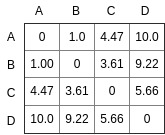
\includegraphics[scale=1]{step1}  
    \caption[Gambar matriks jarak]{Gambar matriks jarak} 
    \label{fig:step1} 
\end{figure}

Jarak antara \textit{cluster} $A$ dan \textit{cluster} $B$ dapat dihitung dengan cara seperti berikut:


\begin{align}
d & = \sqrt{(x_{1} - x_{2})^2+(y_{1} - y_{2})^2} \\
& = \sqrt{(2 - 2)^2+(2 - 3)^2} \\
& = \sqrt{0 + 1} \\
& = \sqrt{1} \\
& = 1 
\end{align}\\


\item Selanjutnya, gabungkan dua \textit{cluster} yang memiliki similaritas tertinggi. Pada contoh ini,  \textit{cluster} $A$ yang dibandingkan terhadap \textit{cluster} $B$ memiliki nilai terkecil yaitu $1$. Similaritas antara kedua \textit{cluster} adalah yang tertinggi. Hasil dari penggabungan kedua cluster dapat dilihat pada Gambar ~\ref{fig:step2}.

\begin{figure}[H]
    \centering  
    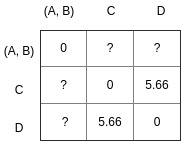
\includegraphics[scale=0.8]{step2}  
    \caption[Gambar penggabungan \textit{cluster}]{Gambar penggabungan \textit{cluster}} 
    \label{fig:step2} 
\end{figure}

\item Setelah itu, matriks jarak harus dikalkulasi ulang untuk mencari similaritas antara \textit{cluster} barunya yaitu ($A$,$B$) dengan yang lainya. Untuk mengkalkulasi ulang antara \textit{cluster} baru dengan \textit{cluster} lainnya, digunakan metode \textit{single linkage}. Pada tahap ini setiap anggota dari cluster ($A$,$B$) akan dihitung jaraknya terhadap \textit{cluster} $C$ dan \textit{cluster} $D$. Nilai minimum akan diambil sebagai hasil perbandingannya karena metode yang digunakan adalah \textit{single linkage}. Berikut adalah contoh perhitungan antara \textit{cluster} ($A$,$B$) dengan \textit{cluster} $C$ menggunakan metode \textit{single linkage}.


\begin{align} 
d(A,C) & = \sqrt{(2 - 2)^2+(4 - 6)^2} \\
& = 4.47 
\end{align}
\begin{align} 
d(B,C) & = \sqrt{(2 - 3)^2+(4 - 6)^2} \\
& = 3.61 
\end{align}\\


Karena nilai 3.61 lebih kecil dari 4.47, maka nilai 3.61 diambil sebagai hasil. Contoh hasil dapat dilihat pada Gambar ~\ref{fig:step3}. 

\begin{figure}[H]
    \centering  
    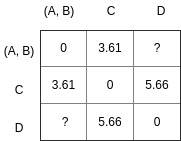
\includegraphics[scale=0.8]{step3}  
    \caption[Gambar hasil rekalkulasi ]{Gambar hasil rekalkulasi} 
    \label{fig:step3} 
\end{figure}

\item Ulangi langkah 2 dan 3 sampai satu \textit{cluster} yang tersisa. Hasil akhir dalam bentuk \textit{dendrogram} dapat dilihat pada Gambar ~\ref{fig:hasild}.

\begin{figure}[H]
    \centering  
    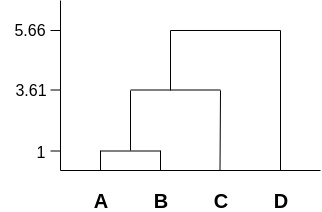
\includegraphics[scale=0.6]{hasild}  
    \caption[Gambar hasil akhir \textit{dendrogram} ]{Gambar hasil akhir \textit{dendrogram}} 
    \label{fig:hasild} 
\end{figure}

\end{enumerate}


\section{Hadoop}

\subsection{Penjelasan Hadoop}

Hadoop dikembangkan oleh Doug Cutting dan Mike Cafarella pada tahun 2005 yang saat itu bekerja di Yahoo. Nama Hadoop diberikan berdasarkan mainan 'Gajah' anak dari Doug Cutting. Hadoop adalah sebuah \textit{framework} atau platform \textit{open source} berbasis Java. Hadoop memiliki kemampuan untuk penyimpanan dan memproses data dengan skala yang besar secara terdistribusi pada {\it cluster}. {\it Cluster} tersebut terdiri dari perangkat keras komoditas ~\cite{alexholmes:04:hip}. Hadoop menggunakan teknologi Google MapReduce dan Google File System (GFS) sebagai fondasinya ~\cite{tomwhite:05:htdg}. Beberapa karakteristik yang dimilki Hadoop adalah sebagai berikut:


\begin{enumerate}

\item {\it Open Source}: Hadoop merupakan proyek {\it open source} dan kodenya bisa dimodifikasi sesuai kebutuhan. 

\item {\it Distributed computing}: Data disimpan secara terdistribusi pada \textit{Hadoop Distributed File System} (HDFS) dan data diproses secara parallel pada node-node di {\it cluster}.

\item {\it Fast}: Hadoop sangat cocok untuk melakukan {\it batch processing} bervolume tinggi karena mampu melakukannya secara parallel.

\item {\it Fault Tolerance}: Hadoop melakukan duplikasi data di beberapa node yang berbeda. Ketika sebuah node gagal memproses data, node yang memiliki duplikat data dapat menggantikanya untuk memproses data tersebut.

\item {\it Reliability}: Kegagalan mesin bukan masalah bagi Hadoop karena adanya duplikasi data.


\item {\it High availability}: Data dapat diambil dari sumber yang lain meskipun kegagalan mesin karena adanya duplikasi data.

\item {\it Scalability}: Hadoop dapat menambahkan node yang lebih banyak kedalam {\it cluster} dengan mudah.

\item {\it Flexibility}: Hadoop dapat menangani data terstruktur maupun data tidak terstruktur. 

\item {\it Economic and cost effective}: Hadoop tidak mahal karena berjalan pada {\it cluster} yang terdiri dari perangkat keras komoditas.

\item {\it Easy to use}: Hadoop mempermudah pengguna dalam merancang program parallel. Hadoop sudah menangani hal-hal terakit komputasi terdistribusi.

\item {\it Data locality}: Algoritma MapReduce akan didekatkan kepada {\it cluter} dan tidak sebaliknya. Ukuran data yang besar lebih sulit untuk dipindahkan dibanding ukuran algoritma yang kecil.


\end{enumerate}

\begin{figure}[H]
    \centering  
    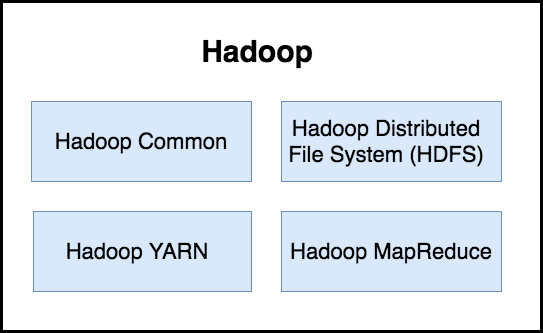
\includegraphics[scale=0.4]{hmodule}  
    \caption[Gambar modul-modul Hadoop ]{Gambar modul-modul Hadoop} 
    \label{fig:hmodule} 
\end{figure}

Bedasarkan gambar diatas (Gambar ~\ref{fig:hmodule}), {\it framework} Apache Hadoop terdiri dari beberapa modul . Modul-modul tersebut membentuk dan membantu untuk memproses data yang bersakala besar. Modul-modul tesebut di antaranya adalah ~\cite{tomwhite:05:htdg}:

\begin{enumerate}
\item Hadoop Common, module ini teridir dari {\it library} dan {\it tools} yang dibutuhkan module Hadoop lainnya.

\item Hadoop Distributed File System (HDFS), sebuah sistem-file terdistribusi milik Hadoop untuk penyimpanan data.

\item Hadoop YARN, {\it resource-management platform} yang bertanggung jawab untuk mengatur sumber daya pada {\it cluster}.

\item MapReduce, sebuah model pemrograman untuk pemrosesan skala besar.

\end{enumerate}

\subsection{Hadoop Distributed File System (HDFS)}

Hadoop Distributed File System (HDFS) adalah sistem file terdistribusi yang dirancang untuk berjalan pada perangkat keras komoditas~\cite{tomwhite:05:htdg}. HDFS berbeda dari sistem file terdistribusi lainnya  karena sifat {\it fault tolerant} yang tinggi dan dirancang untuk digunakan pada perangkat keras biasa. HDFS menyediakan akses \textit{throughput} yang tinggi ke data aplikasi dan cocok untuk aplikasi yang memiliki set data yang besar. HDFS awalnya dibangun sebagai infrastruktur untuk proyek mesin pencari web Apache Nutch.\\

Kegagalan perangkat keras sudah biasa terjadi. HDFS mungkin terdiri dari ratusan atau ribuan mesin server, masing-masing menyimpan bagian dari data {\it file sistem}. Faktanya, ada sejumlah besar komponen dan setiap komponen memiliki probabilitas kegagalan. Hal ini  menandakan bahwa beberapa komponen HDFS selalu tidak berfungsi. Oleh karena itu, deteksi kesalahan dan pemulihan otomatis yang cepat dari sistem adalah tujuan arsitektur inti dari HDFS.\\

\begin{figure}[H]
    \centering  
    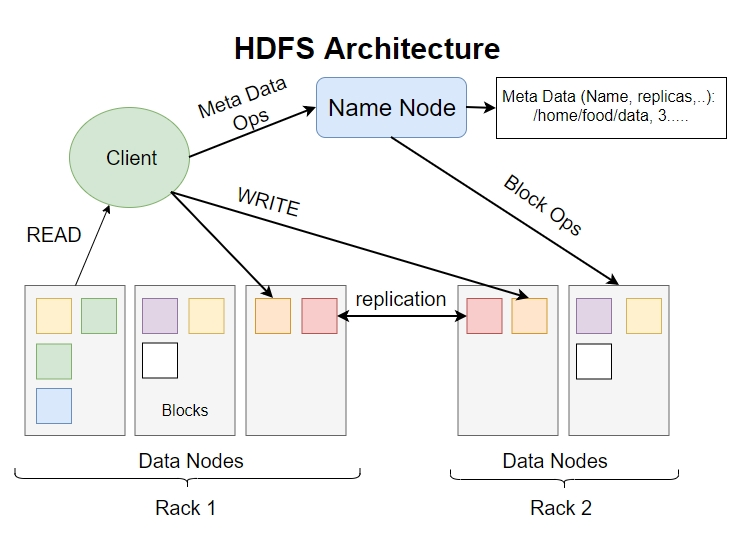
\includegraphics[scale=0.6]{hdfshadoop}  
    \caption[Gambar arsitektur HDFS]{Gambar arsitektur HDFS} 
    \label{fig:hdfshadoop} 
\end{figure}

Hadoop meimplementasikan arsitektur {\it Master Slave} pada komponen primernya yaitu HDFS dan MapReduce ~\cite{tomwhite:05:htdg}. Bedasarkan  (Gambar ~\ref{fig:hdfshadoop}), \textit{master} node atau disebut NameNode bertugas untuk mengatur operasi-operasi seperti membuka, menutup, dan menamakan kembali file atau direktori pada sistem file. Selain itu, NameNode meregulasi akses pengguna terhadap file dan mengatur block mana yang akan diolah oleh DataNode ~\cite{tomwhite:05:htdg}. NameNode membuat semua keputusan terkait replikasi blok. NameNode secara berkala menerima \textit{heart beat} dan \textit{block report} dari masing-masing DataNode di {\it cluster}. \textit{Heart beat} mengimplikasikan bahwa DataNode berfungsi dengan benar.\\
	
{\it Slave} node atau dapat disebut DataNode merupakan pekerja dari HDFS \cite{tomwhite:05:htdg}. DataNode bertangungjawab untuk menjalankan perintah membaca dan menulis untuk sistem file Hadoop. NameNode bisa membuat, menghapus, dan mereplikasi block ketika diberi instruksi dari {\it master node}. DataNode menyimpan dan mengambil blok ketika diperintahkan oleh NameNode. Selain itu, DataNode melaporkan daftar blok-blok yang disimpan kepada NameNode secara rutin.\\ 

HDFS dirancang untuk menyimpan file yang berukuran sangat besar di seluruh mesin dalam {\it cluster} yang besar \cite{tomwhite:05:htdg}. HDFS menyimpan setiap file sebagai blok yang berurutan. semua blok dalam file kecuali blok terakhir memiliki ukuran yang sama. Bisa dilihat pada (Gambar ~\ref{fig:hdfshadoop}) bahwa blok-blok file direplikasi untuk memiliki {\it fault tolerance} yang tinggi. Ukuran blok dan banyaknya replika dapat dikonfigurasi untuk setiap file. Faktor replikasi dapat ditentukan pada waktu pembuatan file dan dapat diubah nantinya.\\

Berikut adalah perintah-peritah dasar yang dapat digunakan untuk HDFS ~\cite{chucklam:06:hia}:

\begin{itemize}
\item Command untuk membuat direktori HDFS untuk penyimpanan file.

\begin{verbatim}
$ hadoop fs -mkdir <dir-path>
\end{verbatim}
 
\item Command untuk melihat daftar konten direktori dari path yang diberikan.

\begin{verbatim}
$ hadoop fs -ls 
\end{verbatim}

\item Command untuk memasukan file atau direktori lokal kepada file sistem destinasi didalam HDFS.

\begin{verbatim}
$ hadoop fs -put <localSrc> <dest> 
\end{verbatim}

\end{itemize}


\subsection{MapReduce}

MapReduce adalah sebuah model pemrograman untuk memproses data berukuran besar secara terdistribusi dan paralel dalam \textit{cluster} yang terdiri atas banyak komputer. Dalam memproses data, secara garis besar MapReduce dapat dibagi dalam dua proses yaitu proses \textit{map} dan proses \textit{reduce} ~\cite{tomwhite:05:htdg}. Setiap fase memiliki pasangan \textit{key-value} sebagai input dan output ~\cite{tomwhite:05:htdg}. Kedua jenis proses ini didistribusikan atau dibagi-bagikan ke setiap komputer dalam suatu cluster dan berjalan secara paralel tanpa saling bergantung satu sama yang lainnya. Proses \textit{map} bertugas untuk mengumpulkan informasi dari potongan-potongan data yang terdistribusi dalam tiap komputer dalam cluster. Hasilnya diserahkan kepada proses Reduce untuk diproses lebih lanjut. Hasil proses Reduce merupakan hasil akhir.\\

\begin{figure}[H]
    \centering  
    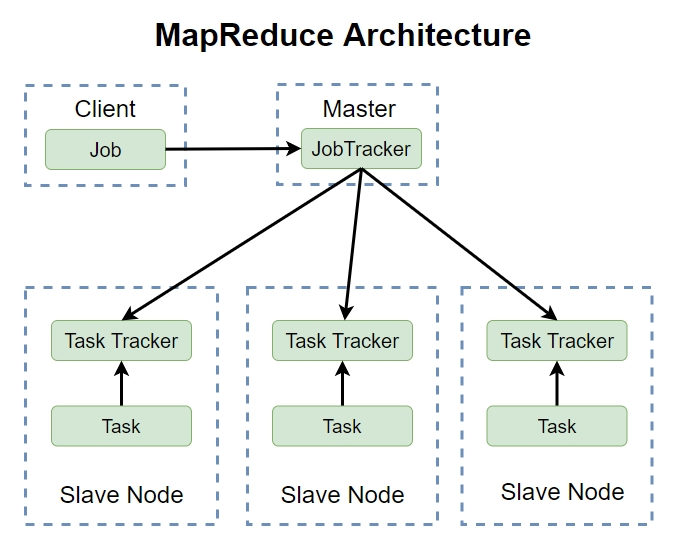
\includegraphics[scale=0.5]{mapreducehadoop}  
    \caption[Gambar arsitektur MapReduce]{Gambar arsitektur MapReduce} 
    \label{fig:mapreducehadoop} 
\end{figure}

Dapat dilihat pada (Gambar ~\ref{fig:mapreducehadoop}) yaitu arsitektur MapReduce. Pada arsitektur ini, {\it master node} disebut JobTracker dan {\it slave node} disebut TaskTracker. JobTracker adalah jembatan antara pengguna dan fungsi \textit{map} maupun \textit{reduce}. Ketika sebuah pekerjaan \textit{map} atau \textit{reduce} diterima oleh JobTracker, pekerjaan tersebut akan dimasukan kedalam antiran. Pekerjaan dalam antrian akan dikerjakan sesuai urutan masuk pekerjaan tersebut. Kemudian, pekerjaan akan ditugaskan kepada TaskTracker oleh JobTracker~\cite{tomwhite:05:htdg}. TaskTracker akan mengeksekusi pekerjaan yang diberikan oleh JobTracker dan mengembalikan laporan progress kepada JobTracker~\cite{tomwhite:05:htdg}.   


\begin{figure}[H]
    \centering  
    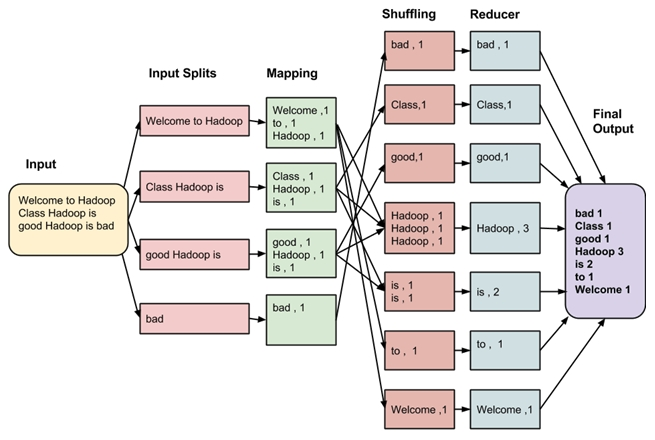
\includegraphics[scale=1]{mpstep}  
    \caption[Gambar proses MapReduce]{Gambar proses MapReduce} 
    \label{fig:mpstep} 
\end{figure}

Bedasarkan (Gambar ~\ref{fig:mpstep}), berikut adalah langkah-langkah proses awal  sampai akhir dari MapReduce:

\begin{enumerate}
\item \textit{Input} dibagi menjadi {\it input split} yang berukuran sama. Setiap \textit{input splits} akan dibuatkan \textit{map task}.

\item Pada fase \textit{map}, data pada setiap \textit{split} akan dihitung berapa banyak kemunculan kata tersebut dan dijadikan pasangan <\textit{word}, \textit{frequency}> sebagai \textit{ouput}.

\item Setelah fase \textit{mapping} adalah fase \textit{shuffling}. Tahap ini mentrasfer \textit{output} dari fase \textit{map} kepada \textit{reducer}. Hasil dari fase \textit{map} akan dikelompokan berdasarkan \textit{key} dan dibagi di antara \textit{reducer}. Dalam contoh ini, kata-kata yang sama disatukan bersama dengan frekuensi masing-masing.


\item Terakhir adalah fase \textit{reduce} dimana \textit{ouput} dari \textit{shuffling} akan dikumpulkan. Nilai-nilai dari fase \textit{shuffling} akan digabungkan menjadi sebuah \textit{output}. \textit{Output} akan disimpan pada HDFS.

\end{enumerate}

\subsection{YARN}

Apache YARN (Yet Another Resource Negotiator) adalah pengatur sumber daya dari \textit{cluster} Hadoop. YARN bertujuan untuk memisahkan fungsionalitas antara pengaturan sumber daya dan penjadwalan pekerjaan. YARN memiliki dua tipe \textit{daemon} yaitu \textit{Resource Manager} dan \textit{Node Manager}~\cite{tomwhite:05:htdg}.  \textit{Resource Manager} bertugas untuk mengatur sumber daya di seluruh \textit{cluster} dan \textit{Node Manager} yang berjalan pada \textit{node}. \textit{Node Manager} bertugas untuk menjalankan dan memantau \textit{container}~\cite{tomwhite:05:htdg}. \textit{Container} bertugas untuk mengeksekusi proses aplikasi yang spesifik.

\begin{figure}[H]
    \centering  
    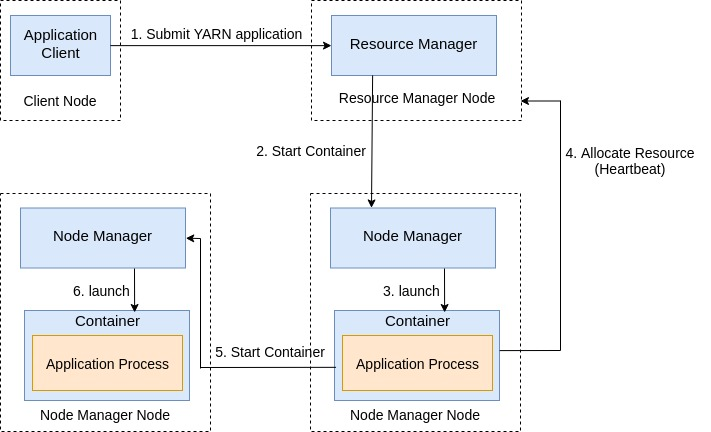
\includegraphics[scale=0.6]{yarn}  
    \caption[Gambar proses menjalankan applikasi pada YARN]{Gambar roses menjalankan applikasi pada YARN} 
    \label{fig:yarn} 
\end{figure}

Berikut adalah Gambar ~\ref{fig:yarn} yang mengabarkan langkah-langkah proses ketika mengjalankan aplikasi pada YARN. Untuk menjalankan applikasi pada YARN, \textit{client} akan meminta \textit{Resource Manager} untuk menjalankan proses aplikasi \textit{master} (langkah 1). Kemudian, \textit{Resource Manager} akan mencari \textit{Node Manager} yang bisa menjalankan applikasi \textit{master} dalam sebuah \textit{container} (langkah 2 dan 3). Ketika aplikasi \textit{master} sudah berjalan, aplikasi \textit{master} bisa melakukan komputasi pada \textit{container} dan mengembalikan hasil kepada \textit{client}. Selain itu, aplikasi \textit{master} bisa saja meminta sumber daya tambahan (langkah 4) dan menggunakan sumber daya tersebut untuk komputasi terdistribusi (langkah 5 dan 6).\\

\section{Spark}

\subsection{Pembahasan Umum Spark}

Apache spark adalah sebuah {\it cluster computing platform} dirancang untuk kecepatan dan {\it general-purpose}~\cite{holdenkarau:07:ls}. Spark dirancang bedasarkan model MapReduce yang populer untuk memberikan dukungan yang efisien kepada banyak tipe komputasi, termasuk {\it interactive query}, dan {\it stream processing} ~\cite{holdenkarau:07:ls}. Kecepatan merupakan kunci dalam memproses data set yang besar, perbedaan waktu dalam eksplorasi data bisa dari beberapa menit sampai beberapa jam tergantung pada kecepatan. Salah satu fitur utama Spark yang ditawarkan adalah kemmapuannya untuk melakukan {\it in memory computations}~\cite{holdenkarau:07:ls}. Selain itu, sistem Spark lebih efisien daripada MapReduce dalam menjalankan applikasi yang rumit pada disk.\\


Pada sisi {\it general-purpose}, Spark dirancang untuk mencakup berbagai beban kerja yang sebelumnya diperlukan sistem terdistribusi terpisah, termasuk aplikasi \textit{batch}, {\it iterative algorithms}, {\it interactive query}, dan \textit{streaming}. Dengan mendukung beban kerja tersebut di mesin yang sama, Spark membuat pekerjaan lebih mudah dan murah untuk menggabungkan pemrosesan yang berbeda jenis. Dengan begitu, Spark mengurangi beban dalam merawat \textit{tools} yang terpisah.\\

Spark di desain agar sangat mudah diakses dengan memberikan API sederhana untuk Python, Java, Scala, dan SQL~\cite{holdenkarau:07:ls}. Spark dengan mudah berintegrasi dengan tools {\it Big Data} lainnya, terutama Hadoop. Spark bisa berjalan pada Hadoop {\it cluster} dan mengakses sumber data Hadoop mana saja.\\

\subsection{Komponen Spark}



Spark memiliki beberapa komponen yang terintegrasi dengan erat. Sebagai {\it core}, Spark adalah "mesin komputasi" yang bertanggung jawab untuk penjadwalan, distribusi, dan pemantauan aplikasi yang terdiri dari banyak task-task komputasi tersebar di banyak pekerja, mesin, atau {\it cluster}~\cite{holdenkarau:07:ls}. Karena {\it core engine} dari Spark sangat cepat dan dirancang untuk tujuan umum, Spark menjalankan banyak komponen di level yang lebih tinggi untuk menangani berbagai macam pekerjaan khusus seperti SQL atau {\it machine learning}~\cite{holdenkarau:07:ls}. Komponen-komponen ini dirancang untuk saling beroperrasi dengan erat, Spark membiarkan pengguna untuk menggabungkan komponen seperti {\it library} dalam suatu proyek perangkat lunak.\\

\begin{figure}[H]
    \centering  
    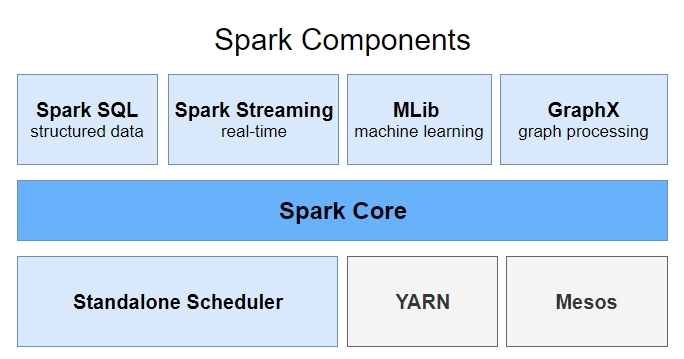
\includegraphics[scale=0.6]{sparkcomponent}  
    \caption[Gambar komponen pada Spark]{Gambar komponen pada Spark} 
    \label{fig:sparkcomponent} 
\end{figure}

Bedasarkan (Gambar ~\ref{fig:sparkcomponent}), Spark memiliki beberapa komponen sebagai berikut:

\begin{itemize}

\item Spark Core:
Spark Core berisi fungsi-fungsi dasar Spark, termasuk komponen untuk tugas penjadwalan, manajemen memori, pemulihan kesalahan, berinteraksi dengan sistem penyimpanan,
dan banyak lagi ~\cite{holdenkarau:07:ls}. Spark Core memiliki banyak API \textit{resilient distributed datasets}(RDD), yang merupakan abstraksi pemrograman utama Spark ~\cite{holdenkarau:07:ls}. RDD mewakili suatu koleksi \textit{item} yang didistribusikan di banyak node komputasi yang dapat dimanipulasi
secara parallel~\cite{holdenkarau:07:ls}. Spark Core menyediakan banyak API untuk membangun dan memanipulasi ini
koleksi. 

\item Spark SQL: Spark SQL adalah sebuah modul untuk bekerja dengan data yang terstuktur module ~\cite{holdenkarau:07:ls}. Modul ini memungkinkan melakukan kueri pada data terstrukut melalui SQL serta varian Apache Hive dari SQL disebut Hive Query Language (HQL) dan mendukung banyak sumber data, termasuk tabel Hive, Parket, dan JSON. Selain menyediakan antarmuka SQL untuk Spark, Spark SQL memungkinkan \textit{developer} untuk memadukan kueri SQL dengan manipulasi data terprogram yang didukung oleh RDD pada Python, Java, dan Scala, semua dalam satu aplikasi, sehingga menggabungkan SQL dengan analitik yang rumit. Integrasi ketat dengan lingkungan komputasi yang kaya disediakan oleh Spark membuat Spark SQL tidak seperti gudang data \textit{open source} lainnya.

\item Spark Streaming: Spark Streaming adalah komponen Spark yang memungkinkan pemrosesan data dari \textit{live streaming} ~\cite{holdenkarau:07:ls}. Contoh \textit{data steam} termasuk file log yang dihasilkan oleh server web produksi, atau antrian pesan yang berisi pembaruan status yang diposting oleh pengguna layanan web. Spark Streaming menyediakan API yang mirip dengan  Spark Core’s RDD API untuk memanipulasi aliran data. Hal ini membuat \textit{developer} mudah memplajari proyek dan berpindah antar aplikasi yang memanipulasi data yang disimpan dalam memori, pada disk, atau tiba dalam \textit{real time}. Di balik API-nya, Spark Streaming dirancang untuk menyediakan tingkat toleransi kesalahan, throughput, dan skalabilitas yang sama seperti Spark Core.

\item MLlib: Spark hadir dengan \textit{library} yang berisi fungsi pembelajaran mesin secara umum (ML), \textit{library} ini disebut MLlib. MLlib menyediakan beberapa jenis algoritma pembelajaran mesin, termasuk klasifikasi, regresi, pengelompokan, dan penyaringan kolaboratif, serta pendukung
fungsionalitas seperti \textit{model evaluation} dan \textit{data import} ~\cite{holdenkarau:07:ls}. MLlib juga menyediakan
beberapa \textit{lower-level} ML \textit{primitives}, termasuk \textit{generic gradient descent optimization
algorithm}.

\item GraphX: GraphX adalah sebuah \textit{library} untuk memanipulasi grafik dan melakukan \textit{graph-parallel computations} ~\cite{holdenkarau:07:ls}. Seperti Spark Streaming dan Spark SQL, GraphX ​​memperluas API Spark RDD, memungkinkan kita untuk membuat \textit{directed graph} dengan\textit{ arbitrary propertiesi} yang melekat pada setiap \textit{vertex} dan \textit{edge}. GraphX ​​juga menyediakan berbagai operator untuk memanipulasi grafik dan memiliki library yang penuh dengan \textit{graph algorithms} yang umum seperti PageRank dan \textit{triangle counting}.

\item Cluster Managers: Spark dirancang untuk dapat ditambah secara efisien dari satu hingga ribuan node komputasi. Untuk mencapai hal ini dan memaksimalkan fleksibilitas, Spark dapat menjalankan lebih dari satu variasi manajer \textit{cluster} seperti Hadoop YARN, Apache Mesos, \textit{simple
cluster manager} pada diri Spark sendiri yang disebut \textit{Standalone Scheduler}.\\

\end{itemize}

\subsection{Tiga Cara Membangun Spark di Atas Hadoop}

\begin{figure}[H]
    \centering  
    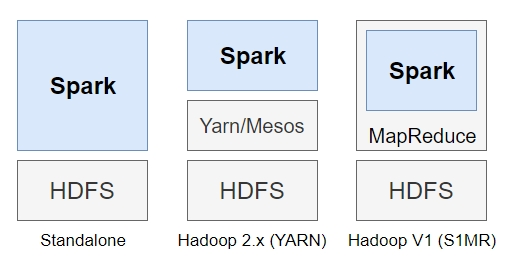
\includegraphics[scale=0.6]{sparkins}  
    \caption[Gambar beberapa cara instalasi Spark]{Gambar beberapa cara instalasi Spark} 
    \label{fig:sparkins} 
\end{figure}

Ada tiga cara untuk meinstalasi Spark bedasarkan (Gambar ~\ref{fig:sparkins}) diatas, ketiga cara tersebut akan dijelaskan dibawah:

\begin{itemize}

\item \textit{Standalone}: Spark \textit{standalone} berarti Spark menempati tempat di atas HDFS (Hadoop Distributed File System) dan ruang dialokasikan untuk HDFS, secara eksplisit. Spark dan MapReduce akan berjalan berdampingan untuk mencakup semua pekerjaan percikan di cluster ~\cite{holdenkarau:07:ls}.

\item Hadoop Yarn: Spark berjalan pada Yarn tanpa perlu pra-instalasi atau akses root ~\cite{holdenkarau:07:ls}. Cara ini membantu mengintegrasikan Spark ke dalam ekosistem Hadoop atau Hadoop stack. Cara ini memungkinkan komponen lain untuk berjalan di atas tumpukan.

\item Spark pada MapReduce: Spark pada MapReduce digunakan untuk menjalankan job-job pada spark selain untuk \textit{standalone deployment} ~\cite{holdenkarau:07:ls}. Dengan adanya SIMR, pengguna dapat memulai Spark dan menggunakan \textit{Spark Shell} tanpa akses administratif.\\

\end{itemize}

\subsection{Resilient Distributed Datasets (RDD)}

Resilient Distributed Datasets (RDD) adalah struktur data dasar Spark. RDD adalah koleksi benda-benda yang didistribusikan secara permanen. Setiap dataset dalam RDD dibagi menjadi beberapa partisi yang dapat dikomputasi pada node yang berbeda pada \textit{cluster} ~\cite{holdenkarau:07:ls}. RDD dapat berisi jenis objek Python, Java, atau Scala, termasuk kelas yang ditentukan pengguna. Spark memanfaatkan konsep RDD untuk mencapai operasi MapReduce yang lebih cepat dan efisien. ~\cite{holdenkarau:07:ls}\\

Secara umun, RDD adalah kumpulan \textit{read-only, partitioned collection} dari \textit{records}. RDD dapat dibuat melalui operasi deterministik dari data pada penyimpanan yang stabil atau RDD lainnya ~\cite{holdenkarau:07:ls}. RDD adalah kumpulan elemen \textit{fault tolerance} yang dapat dioperasikan secara paralel.\\


\textit{Data sharing} pada MapReduce lebih lambat dibanding RDD  karena replikasi, serialisasi, dan disk IO. Sebagian besar aplikasi Hadoop menghabiskan lebih dari 90 persen waktunya untuk melakukan operasi \textit{read-write} keapda HDFS.\\

Untuk menangani masalah tersebut, dibuatlah \textit{framework} khusus disebut Apache Spark. Ide utama dari Spark adalah RDD, Spark mendukung \textit{in-memory computation}. Spark menyimpan status memori sebagai objek di seluruh pekerjaan dan objek dapat dibagi di antara \textit{jobs}. \textit{Data sharing} dalam memori lebih cepat 10 hingga 100 kali lipat dibanding \textit{network} atau \textit{disk}.\\

Berikut adalah sifat-sifat dari RDD :
\begin{itemize}

\item \textit{In Memory}: Data pada RDD disimpan pada memori sebesar mungkin dan selama mungkin.

\item \textit{Partitioned}: \textit{records} dipartisi dan didistribusikan kepada \textit{node}-\textit{node} di dalam \textit{cluster}.

\item \textit{Typed}: RDD memiliki tipe data seperti RDD[Long], RDD[String] dan tipe data lainya.

\item \textit{Lazy evaluation}: Data didalam RDD tidak akan tersedia atau berubah sampai sebuah perintah \textit{action} telah dieksekusi.

\item \textit{Immutable}: RDD yang telah dibuat tidak dapat berubah. Meskipun demikian, RDD
dapat ditransformasi menjadi sebuah RDD baru dengan melakukan perintah \textit{transformation}
pada RDD.

\item \textit{Parallel}: RDD dapat dioperasikan secara pararel.

\item \textit{Cacheable}: Pengguna dapat memilih RDD mana yang akan dipakai kembali dan memilih tempat penyimpanan yaitu memori atau disk. Dengan begitu, data dapat di akses lebih cepat untuk permintaan selanjutnya.\\

\end{itemize}

Ada dua cara untuk membuat sebuah RDD. Cara pertama adalah dengan memuat dataset eksternal~\cite{holdenkarau:07:ls}. Sedangkan cara alternatif adalah dengan mendistribustikan sebuah koleksi objek seperti \textit{list} atau \textit{set}~\cite{holdenkarau:07:ls}. Ketika sebuah RDD telah dibuat, ada dua tipe operasi yaitu \textit{transformations} dan \textit{actions} yang bisa dilakukan RDD. \textit{Transformations} membuat RDD baru dari RDD sebelumnya~\cite{holdenkarau:07:ls}. Berbeda dengan \textit{tranformations}, \textit{actions} mengembalikan nilai hasil komputasi bedasarkan RDD~\cite{holdenkarau:07:ls}. Hasil dari \textit{actions} akan dikembalikan kepada \textit{driver program} atau di simpan pada penyimpanan eksternal seperti HDFS. \\

Berikut adalah contoh pembuatan RDD dari sumber eksternal dan koleksi objek:
\begin{itemize}

\item
\begin{verbatim}
Contoh pembuatan RDD dari sumber eksternal.
val lines = sc.textFile("/path/to/README.md")
\end{verbatim}

\item
\begin{verbatim}
Contoh pembuatan RDD dari koleksi objek.
val lines = sc.parallelize(["a", "b", "c", "d", "e"])\\
\end{verbatim}

\end{itemize}


\textit{Transformations} pada RDD adalah sebuah operasi yang menerima RDD sebagi masukan dan mengembalikan satu atau lebih RDD baru. RDD masukan tidak berubah karena sifat RDD adalah \textit{immutable} yang berarti tidak bisa diubah ketika dibuat. \textit{Transformations} bersifat \textit{lazy}, \textit{transformation} tidak langsung dieksekusi, Spark akan mencatat \textit{tranfomartion} apa saja yang dilakukan pada RDD awal. \textit{Transformations} akan dieksekusi ketika sebuah \textit{actions} dipanggil.\\

Berikut adalah contoh \textit{filter} \textit{transformation} di Scala. \textit{Filter} digunakan untuk menyaring elemen-elemen yang sesuai dengan kriteria yang ditentukan. Pada kasus ini, filter akan mengambilkan baris-baris yang memiliki kata \textit{error}.
\begin{verbatim}
val inputRDD = sc.textFile("log.txt") 
val errorsRDD = inputRDD.filter(line => line.contains("error"))
\end{verbatim}

Berikut adalah Tabel~\ref{tab:trans} berisi daftar \textit{transformations} yang umum pada Spark:

\begin{table}[H] 
	\centering 
	\caption{Tabel transformastions}
	\label{tab:trans}
	\begin{tabular}{p{6cm}p{9cm}}
		\toprule[1.5pt]
\hline
		 \textbf{\textit{Transformations}} & Penjelasan \\
\hline
\midrule

\hline
\textbf{map}(func) & Mengembalikan dataset terdistribusi baru yang dibentuk dengan melewatkan setiap elemen melalui fungsi func. \\
\hline

\textbf{filter}(func) & Mengembalikan dataset baru yang dibentuk dengan memilih elemen-elemen yang mengembalikan nilai true dari fungsi func. \\
\hline

\textbf{flatMap}(func) & Mirip dengan \textit{map}, tetapi setiap \textit{item input} dapat dipetakan ke nol atau lebih \textit{item output}. \\
\hline


\textbf{union}(otherDataset) & Mengembalikan \textit{dataset} baru yang mengandung \textit{element} dari sumber dan \textit{dataset}lainnya.\\

\hline
\textbf{intersection}(otherDataset) & Mengembalikan \textit{dataset} baru yang berisi potongan \textit{element} dari sumber dan \textit{argument}.\\ 

\hline
\textbf{distinct}([numPartitions]) & Mengembalikan \textit{dataset} baru yang mengandung \textit{element} yang unik dari \textit{dataset} sumber.\\

\hline
\textbf{groupByKey}([numPartitions]) & Mengembalikan \textit{dataset} baru bertipe \textit{pairs}  (K, Iterable<V>) dari sumber \textit{dataset} bertipe (K, V).\\


\hline
\textbf{groupByKey}(func,[numPartitions]) & Mengembalikan \textit{dataset} baru berupa \textit{pairs} (K, V) yang sudah diagregasi bedasarkan \textit{key} dan fungsi \textit{reduce} yang diberikan.\\

\hline
\textbf{sortByKey}([ascending], [numPartitions]) & Mengembalikan \textit{dataset} baru berupa \textit{pairs}  (K, V) yang terurut secara menaik atau menurun badsarkan parameter boolean yang diberikan.\\

\hline
\textbf{join}(otherDataset, [numPartitions]) & Mengembalikan gabungan \textit{dataset} berupa \textit{pairs}  (K, V) dan (K, W) menjadi \textit{pairs} (K, (V,W)).\\

\hline
\textbf{cogroup}(otherDataset, [numPartitions]) & Mengembalikan \textit{dataset} berupa \textit{tuples}  (K, (Iterable<V>, Iterable<W>)) dari \textit{pairs} (K, V) dan (K, W).\\

\hline
\textbf{cartesian}(otherDataset) & Mengembalikan \textit{dataset} berupa \textit{paris}  (T, U) dari \textit{dataset} T dan U.\\

\hline


\bottomrule
		
	\end{tabular} 
\end{table}

Berikut adalah contoh operasi \textit{action} pada RDD. Pada contoh ini, fungsi \textit{reduceByKey} digunakan untuk menghitung jumlah kata yang ada.

\begin{verbatim}
val lines = sc.textFile("data.txt") 
val pairs = lines.map(s => (s, 1))
val counts = pairs.reduceByKey((a, b) => a + b)
\end{verbatim}

\textit{Actions} merupakah operasi yang mengembalikan sebuah nilai kepada \textit{driver program} atau tempat penyimpanan eksternal. Untuk mengembalikan sebuah nilai, kita bisa menggunakan take(), count(), collect(), dan \textit{actions} lainya. Operasi take() digunakan untuk mengambil sebagian kecil \textit{element} pada RDD. Ketika menggunakan collect(), memori pada satu komputer harus cukup untuk menampung seluruh \textit{dataset} ~\cite{holdenkarau:07:ls}. Operasi tersebut sebaiknya digunakan pada \textit{dataset} yang berukuran kecil. \textit{Dataset} yang berukuran besar dapat disimpan pada tempat penyimpanan eksternal. Setiap kali sebuah \textit{actions} dipanggil, seluruh RDD akan dikomputasi dari akarnya. Untuk mencapai efisiensi yang lebih tinggi, bisa dilakukan \textit{persist} terhadap \textit{intermediate results}. \\

Berikut adalah Tabel~\ref{tab:actions} berisi daftar \textit{actions} yang umum pada Spark:


\begin{table}[H] 
	\centering 
	\caption{Tabel Actions}
	\label{tab:actions}
	\begin{tabular}{p{6cm}p{9cm}}
		\toprule[1.5pt]
\hline
		 \textbf{\textit{Actions}} & Penjelasan \\
\hline
\midrule

\hline
\textbf{reduce}(func) & Mengagregasikan seluruh \textit{element} pada \textit{dataset} menggunakan fungsi yang diberikan pada \textit{parameter}. \\

\hline
\textbf{collect}() & Mengembalikan seluruh \textit{dataset} sebagai array kepada \textit{driver program}. \\

\hline
\textbf{count}() & Mengembalikan jumlah \textit{element} pada \textit{dataset}. \\

\hline
\textbf{first}() & Mengembalikan \textit{element} pertama pada \textit{dataset}. \\

\hline
\textbf{take}(n) & Mengembalikan sebuah array dengan n jumlah \textit{element} pertama dari \textit{dataset}.\\

\hline
\textbf{takeOrdered}(n, [ordering]) & Mengembalikan sebuah array dengan n jumlah \textit{element} pertama dari \textit{dataset} secara terurut. \\

\hline
\textbf{saveAsTextFile}(path) & Menyimpan \textit{dataset} sebagai \textit{text file} pada direktori yang ditentukan. \\

\hline
\textbf{saveAsSequenceFile}(path) & Menyimpan \textit{dataset} sebagai Hadoop SequenceFile pada direktori yang ditentukan.\\

\hline
\textbf{saveAsObjectFile}(path) & Menyimpan \textit{dataset} sebagai format yang sederhana menggunakan Java Serialization pada direktori yang ditentukan.\\

\hline
\textbf{countByKey}() & Menjumlahkan \textit{pairs} (K, V) bedasarkan \textit{key} dan mengembalikan sebuah \textit{pairs} berisi (K, int). \\

\hline
\textbf{foreach}(func) & Memproses setiap \textit{element} pada \textit{dataset} menggunakan fungsi func yang diberikan. \\

\hline


\bottomrule
	\end{tabular} 
\end{table}

\section{Scala}


Scala adalah sebuah bahasa pemrograman yang diciptakan oleh Martin Odersky yaitu seorang Profesor di Ecole Polytechnique Federale de Lausanne, sebuah kampus di Lausanne, Swiss. Kata Scala sendiri merupakan kependekan dari "Scalable Language". Karena Scala berjalan diatas Java Virtual Machine (JVM), Scala memiliki performa yang relatif cepat dan juga memungkinkan untuk menggabungkan kode di Scala dengan di Java. Termasuk library, framework dan tool yang ada di Java, bisa gunakan di Scala. Scala menggabungkan konsep Object Oriented Programming (OOP) yang dikenal di Java dengan konsep Functional Programming (FP). Adanya konsep FP inilah yang menjadikan Scala sangat ekspresif, nyaman dan menyenangkan untuk digunakan. \\

Perintah scalac digunakan untuk mengkompilasi program Scala dan akan menghasilkan beberapa file kelas di direktori saat ini. Salah satunya akan disebut file .class. Ini adalah bytecode yang akan berjalan di Java Virtual Machine (JVM) dengan menggunakan perintah scala. \\

\subsection{Expressions}

suatu \textit{ekspressions} adalah pernyataan atau argumen yang dapat dikomputasi.

\begin{verbatim}
1 + 1
2 + 2 
\end{verbatim}


\textit{Ekspressions} dapat dikembalikan dengan perintah println.

\begin{verbatim}
println(1)
println(100) // 100
println(1 + 1) // 2
println("Hi!") // Hi!
\end{verbatim}


\textit{Ekspressions} atau pernyataan seperti diatas dapat disimpan dalam sebuah \textit{variable}. Ada dua jenis \textit{variable} di Scala yaitu val dan var. Setelah val diinisialisasi, val tidak dapat diisi kembali artinya isi dari val tidak dapat diubah.

\begin{verbatim}
val x = 2 + 5
val x = 10 //tidak akan di compile 
val y = 7
val coba:Int = 200 
\end{verbatim}

\textit{variable} mirip dengan value, tetapi nilai \textit{variable} dapat di isi kembali.

\begin{verbatim}
var x = 2 + 2 
x = 4 
println(x) // 4 
x = 7 
println(x) // 7 
\end{verbatim}

Secara eksplisit kita bisa menyatakan tipe dari sebuah var atau val dengan cara:

\begin{verbatim}
var x: Int = 1 + 1 // Int merupakan tipe dari variable x
val y: Long = 987654321 // Long merupakan tipe dari variable y
val z: Char = 'a' // Char merupakan tipe dari variable z
\end{verbatim}

\subsection{Blocks}

Block digunakan untuk menggabungkan \textit{expressions}. Berikut adalah contoh \textit{block}:

\begin{verbatim}
println({
    val x = 1 + 1
    x + 1
}) // 3 
\end{verbatim}

\subsection{Loop dan Conditional}

loop adalah struktur pengulangan yang memungkinkan untuk menulis secara efisien suatu loop yang perlu dieksekusi sejumlah kali. Ada berbagai bentuk loop dalam Scala yang dijelaskan di bawah ini: 

\begin{verbatim}
for( var x <- Range ){
   statement(s);
}

var x = 0
while (x < 10) {
    println(x)
    x += 1
}
\end{verbatim}

Percabangan adalah pengujian sebuah kondisi. Jika kondisi yang diuji tersebut terpenuhi, maka program akan menjalankan pernyataan-pernyataan tertentu. Jika kondisi yang diuji salah, program akan menjalankan pernyataan yang lain. Berikut adalah contoh percabangan dalam bahasa Scala:

\begin{verbatim}
if( x < 20 ){
    println("This is if statement");
}

if( x < 20 ){
    if( x< 5) {
        println("smallest");
    }
}

if( x < 10 ){
    println("This is bigger");
} else { 
    println("This is smaller");
}

if( x == 1 ){
    println("1");
} else if (x == 2){ 
    println("2");
}
\end{verbatim}


\subsection{Functions}

\textit{Functions} adalah \textit{expression} yang mempunyai atau menerima parameter. Sebuah function yang tidak memliki nama disebut \textit{anonymous function}. Berikut adalah contoh \textit{anonymous function} dan \textit{function} biasa. Sebuah \textit{function} dapat memiliki lebih dari satu parameter.

\begin{verbatim}
(x: Int) = > x + 1 // Anonymous function 

val addOne = (x: Int) => x + 1 // function biasa 
println(addOne(2)) // 3 

val add = (x: Int, y: Int) => x + y 
println(add(1, 2)) // 3 
\end{verbatim}

Pada sisi sebelah kiri tanda => adalah parameter-parameter sebuah \textit{function}, pada sisi  sebelah kanan merupakan expresi-expresi yang melibatkan parameter tersebut. \\


\subsection{Methods}

\textit{Method} sangat mirip dengan \textit{functionn}, tetapi \textit{method} memiliki beberapa perbedaan. Method harus di definisikan dengan kata kunci def, diikuti dengan nama \textit{method}, parameter-parameter dari \textit{method} tersebut, tipe kembalian \textit{method}, dan isi dari \textit{method} tersebut. 

\begin{verbatim}
def add(x: Int, y: Int): Int = x + y 
println(add(1, 2)) // 3 
\end{verbatim}

Method bisa mempunyai lebih dari satu parameter. 

\begin{verbatim}
def addThenMultiply(x: Int, y: Int)(multiplier: Int): Int = (x + y) * multiplier 
println(addThenMultiply(1, 2)(3)) // 9 
\end{verbatim}


Method dapt tidak memiliki parameter.

\begin{verbatim}
def name: String = System.getProperty("user.name")
println("Hello, " + name + "!")
\end{verbatim}

Method berbeda dengan functions bisa memiliki \textit{multi-line expressions}

\begin{verbatim}
def getSquareString(input: Double): String = {
    val square = input * input
    square.toString
}
\end{verbatim}

Expresi terakhir dari method menjadi nilai yang akan dikembalikan. Scale memunyai \textit{keyword} return, tetapi sangat jarang digunakan.

\subsection{Class dan Object}

\textit{Class} pada Scala di definisikan dengan kata kunci \textit{class} diikuti dengan namanya dan terakhir adalah \textit{constructor} parameter.

\begin{verbatim}

class Greeter(prefix: String, suffix: String) {
    def greet(name: String): Unit = {
        println(prefix + name + suffix)
    }
}

\end{verbatim}



Berikut adalah cara mendeklarasi objek pada Scala
\begin{verbatim}
val greeter = new Greeter("Hello, ", "!")
greeter.greet("Scala developer")
\end{verbatim}

Objek dapat dianggap sebagai sesuatu instansi yang tunggal pada class itu sendiri. Untuk mendefinisikan objek, digunakan kata kunci \textit{Object}. 

\begin{verbatim}
object IdFactory {
    private var counter = 0

  	def create(): Int = {
        counter += 1
        counter
    }
}

val newId: Int = IdFactory.create()
println(newId) // 1
val newerId: Int = IdFactory.create()
println(newerId) // 2

\end{verbatim}

Main method adalah sebuah pintu masuk dari sebuah program. Java Virtual Machine membutuhkan sebuah main method yang dinamakan main dan menerima satu argument, seubah array bertipe string.\\

Menggunakan \textit{object}, kita bisa mendefinisikan sebuah main method seperti berikut: 

\begin{verbatim}
object Main {
  	def main(args: Array[String]): Unit = {
        println("Hello, Scala developer!")
    }
}
\end{verbatim}

\subsection{Higher Order Function}

Pada bahasa Scala ada yang disebut sebagai Higher Order Function. Higher Order Function merupakan sebuah function yang menerima function lainya sebagai parameter dan mengembalikan sebuah function sebagai hasilnya. Berikut adalah contoh-contoh Higher Order Function:

\begin{verbatim}

val salaries = Seq(20000, 70000, 40000) 
val doubleSalary = (x: Int) => x * 2
val newSalaries = salaries.map(doubleSalary) // List(40000, 140000, 80000)

\end{verbatim}

Kita bisa mempersingkat kode dengan sebuah function anonymous dan langsung dimasukan pada parameter

\begin{verbatim}
val salaries = Seq(20000, 70000, 40000)
val newSalaries = salaries.map(x => x * 2) // List(40000, 140000, 80000)
\end{verbatim}

Kita juga dapat memasukan method pada parameter higher order function, compiler Scala akan mengubah sebuah method menjadi function.


\begin{verbatim}
case class WeeklyWeatherForecast(temperatures: Seq[Double]) {

    private def convertCtoF(temp: Double) = temp * 1.8 + 32 

    def forecastInFahrenheit: Seq[Double] = temperatures.map(convertCtoF) } 
}
\end{verbatim}


Salah satu alasan untuk menggunakan \textit{higher order function} adalah untuk mengurangi kode yang berlebihan. Katakanlah ada beberapa metode yang dapat menaikkan gaji seseorang dengan berbagai faktor. Tanpa membuat \textit{higher order function}, kode akan terlihat seperti berikut:

\begin{verbatim}

object SalaryRaiser {

    def smallPromotion(salaries: List[Double]): List[Double] =
        salaries.map(salary => salary * 1.1)

  	def greatPromotion(salaries: List[Double]): List[Double] =
        salaries.map(salary => salary * math.log(salary))

  	def hugePromotion(salaries: List[Double]): List[Double] =
        salaries.map(salary => salary * salary)
}
\end{verbatim}

Perhatikan bahwa masing-masing dari ketiga method hanya berbeda pada faktor perkalian. Untuk menyederhanakan, kita dapat mengeluarkan kode yang redundan menjadi \textit{higher order function} seperti:

\begin{verbatim}
object SalaryRaiser {

   private def promotion(salaries: List[Double], promoF: Double => Double): List[Double] =
        salaries.map(promotionFunction)  

  	def smallPromotion(salaries: List[Double]): List[Double] =
        promotion(salaries, salary => salary * 1.1)

  	def bigPromotion(salaries: List[Double]): List[Double] =
        promotion(salaries, salary => salary * math.log(salary))

  	def hugePromotion(salaries: List[Double]): List[Double] =
        promotion(salaries, salary => salary * salary)
}
\end{verbatim}





